% !TeX spellcheck = de_CH_frami

\section{Graphen\label{sec:sgwt:graphs}}
\rhead{Graphen}

Unsere Grundlage, auf der wir die SGWT aufbauen wollen, stellen Graphen dar. 
Ein Graph $G$ setzt sich aus Kanten $E$ und Knoten $V$ zusammen.
\begin{equation*}
G = \{V, E\}
\end{equation*}
Eine Kante verbindet dabei jeweils zwei Knoten miteinander.
\begin{equation*}
E = (V_1, V_2)
\end{equation*}

\begin{figure}
    \centering
    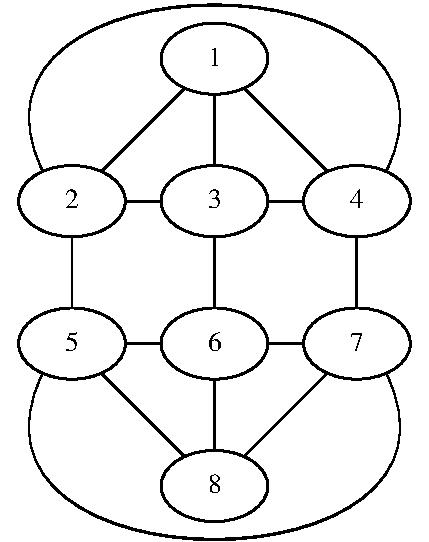
\includegraphics[
        scale=0.7
    ]{papers/sgwt/images/sphere-graph.pdf}
    \caption{Graph Approximation einer Kugel. \label{sgwt:sphere:graph}}
\end{figure}

\begin{figure}
    \centering
    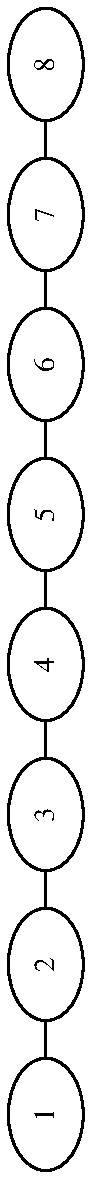
\includegraphics[
        angle=-90,
        origin=c,
        scale=0.7
    ]{papers/sgwt/images/line-graph.pdf}
    \vspace{-200pt}
    \caption{Graph Approximation einer eindimensionalen Funktion. 
    \label{sgwt:line:graph}}
\end{figure}

\begin{figure}
    \centering
    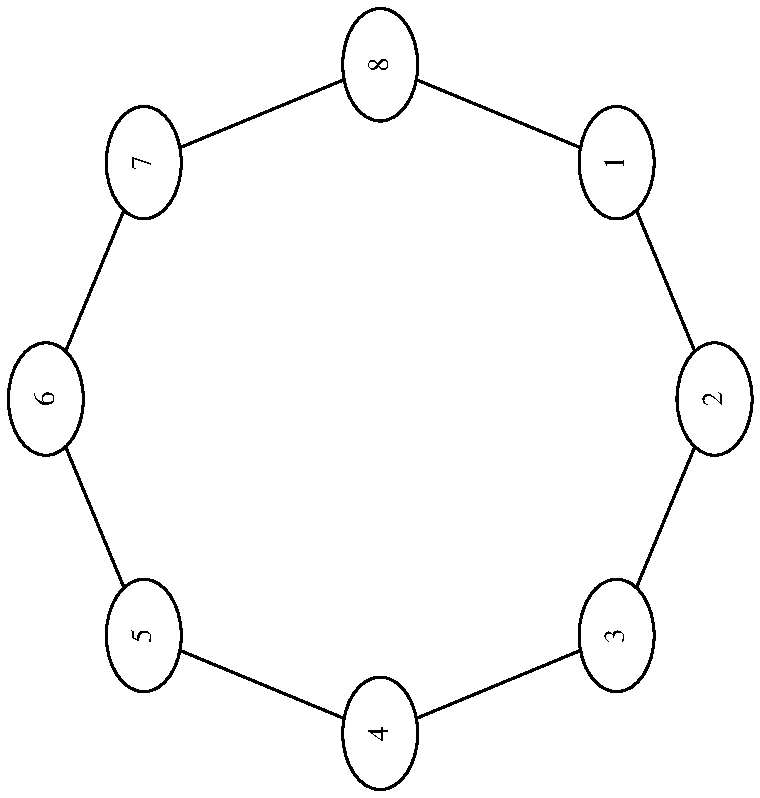
\includegraphics[
        angle=-90,
        origin=c,
        scale=0.7
    ]{papers/sgwt/images/ring-graph.pdf}
    \caption{Graph Approximation einer periodischen eindimensionalen Funktion. 
    \label{sgwt:ring:graph}}
\end{figure}

